%%=============================================================================
%% Methodologie
%%=============================================================================

\chapter{Methodologie}
\label{ch:methodologie}

%% TODO: Hoe ben je te werk gegaan? Verdeel je onderzoek in grote fasen, en
%% licht in elke fase toe welke stappen je gevolgd hebt. Verantwoord waarom je
%% op deze manier te werk gegaan bent. Je moet kunnen aantonen dat je de best
%% mogelijke manier toegepast hebt om een antwoord te vinden op de
%% onderzoeksvraag.
Dit hoofdstuk beschrijft hoe men het best te werk kan gaan in de opzet van een \textit{eenvoudig, kleinschalig blockchain gebaseerd stemsysteem}. Het doel is om een praktische en complete handleiding te vormen, hoofdzakelijk gericht op ontwikkelaars die niet vertrouwd zijn met het ontwikkelen van Ethereum Dapps, noch met het ontwikkelen van cryptografische stemsystemen. 

Gezien de vrij technische aard van deze handleiding wordt er van uit gegaan dat de lezer een algemene voorkennis heeft op het vlak van programmatie en enigszins bekend is met Javascript. Kennis van de taal Solidity wordt niet verondersteld. Tenslotte wordt er veronderstelt dat de lezer over een basis kennis Engels beschikt, daar de volledige code-basis in die taal geschreven is. 

De  verschillende implementatie keuzes die hier wordt gemaakt gebeuren op basis van verschillende concepten en technieken die werden toegelicht in het vorig hoofdstuk. Zo wordt er bijvoorbeeld gekozen voor het Ethereum platform als ontwikkelomgeving op basis van sectie \ref{sec:ethereum-en-smart-contracts} en voor de cryptografie van het zelf-tellende stemprotocol OVNP \autocite{McCorry2017} uit sectie \ref{sec:OVNP}.

In dit hoofdstuk trachten we ook verder antwoord te bieden op enkele van onderzoeksvragen van deze scriptie, metname: 
\begin{itemize}
	\item \textit{wat de praktikaliteit van een blockchain gebaseerd stemsysteem is}
	\item \textit{hoe haalbaar is een blockchain gebaseerd stemsysteem} 
	\item \textit{of er sprake van een onoverkomelijk schaalbaarheidsprobleem}
\end{itemize}

\section{Benodigdheden}
\label{sec:benodigdheden}
	De volgende zaken dienen geïnstalleerd te worden voor men van start kan gaan met het implementeren van een gedecentraliseerde Ethereum blockchain applicatie:
	\begin{itemize}
		\item{Node.js}
		\item{npm}
		\item{Truffle}
		\item{Ganache}
		\item{Metamask}
	\end{itemize}
	Daarnaast heeft men ook nodig:
	\begin{itemize}
		\item{Een IDE code-editor naar keuze met syntax ondersteuning voor Solidity}
		\item{Google Chrome}
	\end{itemize}
	\subsection{Node en npm}
	Node.js is een populaire Runtime-omgeving waarmee Javascript op ieder platform uitgevoerd kan worden, zonder dat daar een browser voor nodig is. Npm is een pakketbeheerder voor Javascript code. Npm zit standaard in Node.js en is `s werelds grootste softwareregister. Open source-ontwikkelaars wereldwijd gebruiken het om pakketten te delen, veel organisaties gebruiken npm om ook hun privéontwikkeling te beheren (\ref{fig:nodejs}).\footnote{Verkregen en vertaald van https://docs.npmjs.com/about-npm/}
	
	Eenmaal node\footnote{node met npm is verkrijgbaar via https://nodejs.org} en npm\footnote{npm is ook apart verkrijgbaar via https://www.npmjs.com/get-npm} geïnstalleerd zijn, verifieert men de installatie via het console-commando: 
	\lstset{language=bash}
	\begin{lstlisting}[numbers=none]
	> node -v
	\end{lstlisting}Bij correcte installatie geeft dit de huidige node versie terug, bijvoorbeeld \textit{v10.15.1}. 
	
	\begin{figure}
		
\includegraphics[width=\linewidth/2]{img/nodejs.png}
		
\includegraphics[width=\linewidth/2]{img/npm.png}
		\caption{De Node.js en npm logo's}
		\label{fig:nodejs}
	\end{figure}
	
	\subsection{Truffle}
	Truffle is een ontwikkelomgeving, testframework en asset pipline, gericht op het versoepelen van het Ethereum ontwikkelproces. Het bevat ook verschillende code-templates die als basis kunnen worden gebruikt om gedecentraliseerde applicaties te ontwikkelen.
	
	Truffle kan eenvoudig geïnstalleerd worden via npm (mits dit  voorgeïnstalleerd is) met het console-commando:
	 \lstset{language=bash}
	\begin{lstlisting}[numbers=none]
	> npm install truffle
	\end{lstlisting}
	\subsection{Ganache}
	Ganache\footnote{Ganache is verkrijgbaar via https://www.trufflesuite.com/ganache} is een applicatie die ontwikkelaars in staat stelt om een private Ethereum-blockchain op te zetten. We gebruiken deze blockchain gedurende de volledige ontwikkelperiode. Op deze manier kan men kosteloos smart-contracts ontwikkelen en testen, als men direct op de Ethereum hoofdketen ontwikkelt is er  immers aan iedere transactie  een kost verbonden. 
	
	Ganache biedt ons  niet enkel een lokale blockchain, het biedt ons ook 10 Ethereum accounts om te gebruiken tijdens het ontwikkelen. Deze accounts hebben adressen die corresponderen met adressen op de lokale Ethereum-blockchain. Elke account is vooraf geladen met 100 nep-ether.
	
	Figuur \ref{fig:ganache-blockchain}: Eenmaal Ganache geïnstalleerd is, open we de applicatie. Door het kiezen van de optie \textit{quickstart} zetten we onmiddellijk een lokale blockchain op. 
	
	\begin{figure}
		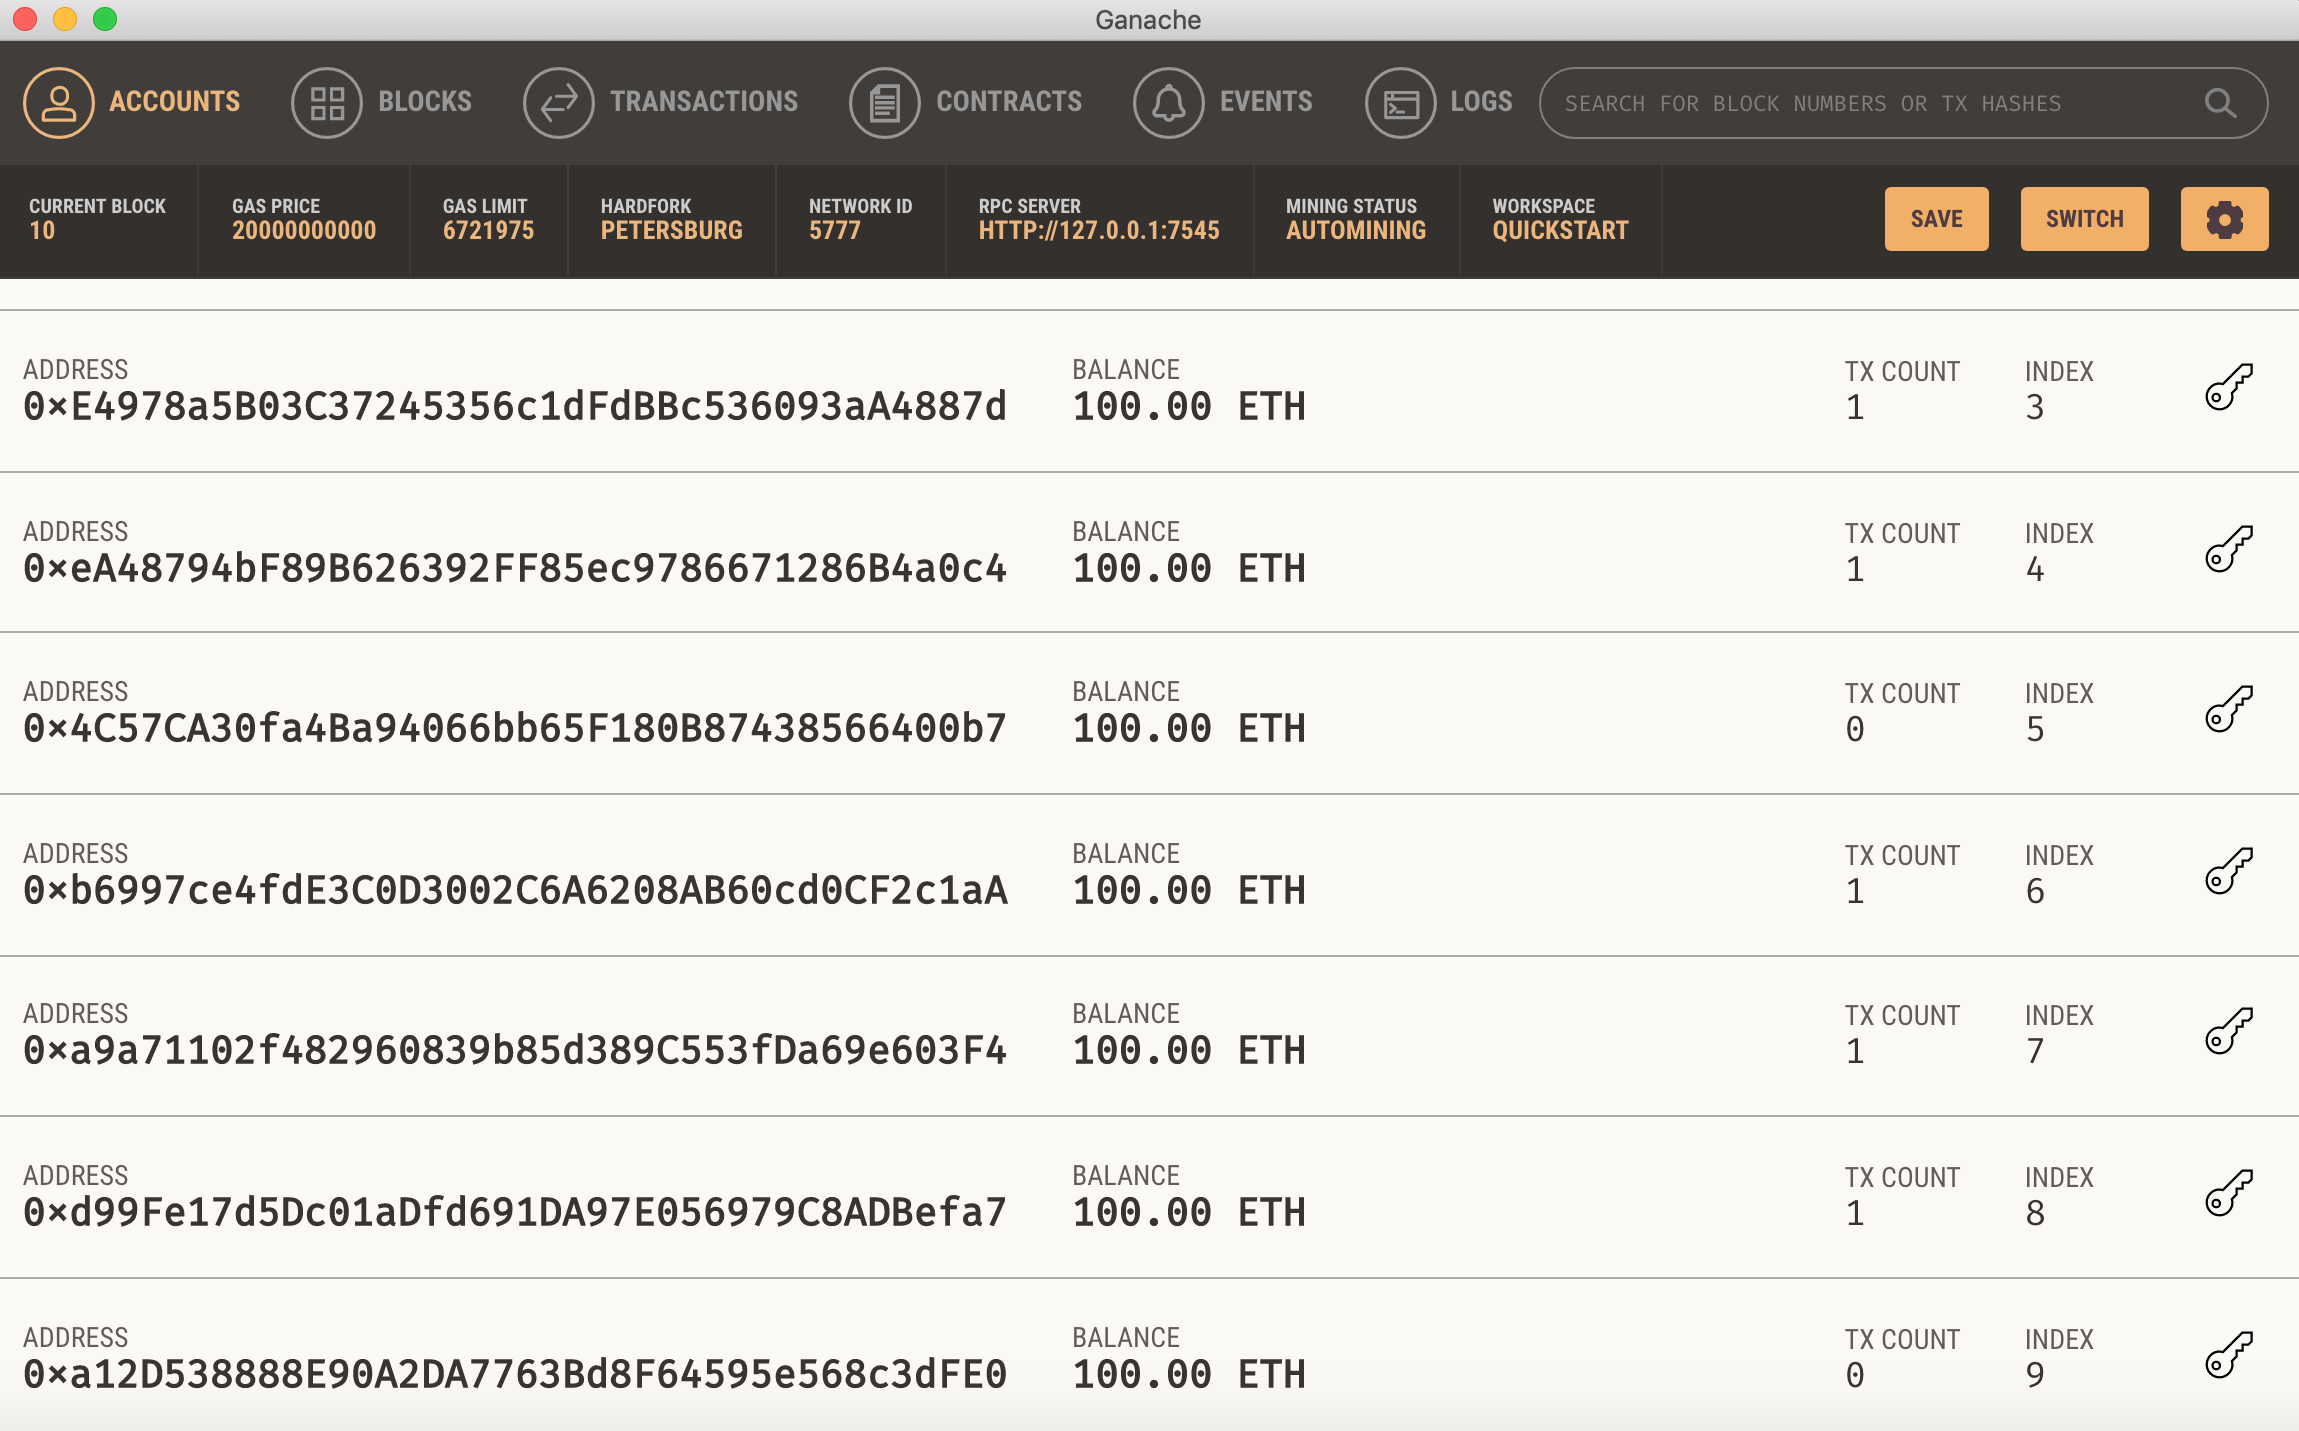
\includegraphics[width=\linewidth]{img/ganache-blockchain.png}
		\caption{Een Lokale blockchain opgezet via Ganache}
		\label{fig:ganache-blockchain}
	\end{figure}
	
	
	\subsection{Metamask}
	Metamask\footnote{Metamask is verkrijgbaar via https://metamask.io of via https://chrome.google.com/webstore} is een Ethereum wallet plugin voor Google Chrome die gebruikers toelaat om transacties van Ethereum dApps uit te voeren in de browser, zonder zelf een node moeten zijn in het netwerk. Door Metamask te installeren hoeft men met andere woorden de volledige blockchain dus niet meer te downloaden. 
	
	Voor deze implementatie is Metamask van cruciaal belang gezien het verantwoordelijk is voor de verificatie van Ethereum accounts. Daarnaast is het ook een zeer handige tool wanneer we onze implementatie in de browser willen testen, het laat ons toe om zeer snel tussen verschillende accounts te verspringen.
	
	Eenmaal de plugin geïnstalleerd is dient men een paswoord te creëren, daarnaast krijgt men ook een fallback sleutel
	
	\begin{figure}
		
\includegraphics[width=\linewidth]{img/metamask-truffle-ganache.png}
		\caption{Truffle, Metamask en Ganache logo's}
		\label{fig:metamask-truffle-ganache}
	\end{figure}
	\newpage
\section{Implementatie Smart Contracts}
	Eenmaal al de verschillende tools en plugins uit sectie \ref{sec:benodigdheden} geïnstalleerd zijn kan men aan het ontwikkelen van smart-contracts beginnen. In de volgende subsecties volgt de implementatie van een blockchain gebaseerd stemsysteem op basis van smart-contracts. Het volledige project kan gevonde worden op Github\footnote{Zie: https://github.com/Ocean97Li/bachelorproef/tree/master/poc/EthereumVote/backend} We beginnen met een simpele implementatie die niet self-tallying is. In een latere sectie zullen we de nodige cryptografie toevoegen om een systeem gelijkaardig aan het Open Network Protocol van  \textcite{McCorry2017} te bekomen.
	\subsection{Opzet Truffle}
	Voor we beginnen met het ontwikkelen van onze smart-contracts moeten we eerst een ontwikkelomgeving opzetten. Voor een vlotte start maken we gebruik van één van de template projecten beschikbaar via Truffle. 
	
	Na te navigeren naar een gewenste directory, gebruikt men het console commando: 
	 \lstset{language=bash}
	\begin{lstlisting}[numbers=none]
	> truffle unbox pet-shop
	\end{lstlisting}
	
	Dit creëert een nieuw project in de huidige directory, we openen het in een code-editor (Bijvoorbeeld VS-code). Figuur \ref{fig:truffle-template} toont de structuur van de genereerde Truffle template. Het project bevat momenteel zowel een back-end gedeelte (smart-contract) als een front-end (een javascript project). 
	
	In deze handleiding zullen we, met het principe van herbruikbaarheid in gedachten, de code opsplitsen in aparte front- en back-end projecten, de folder en inhoud onder \textit{\slash src}, als ook de afbeeldingen \textit{box-img-lg.png} en \textit{box-img-sm.png} mogen dus uit dit project verwijderd worden.
	
	Het project kan nu als start-template worden gebruikt voor onze implementatie.
	
	\begin{figure}
		\centering
		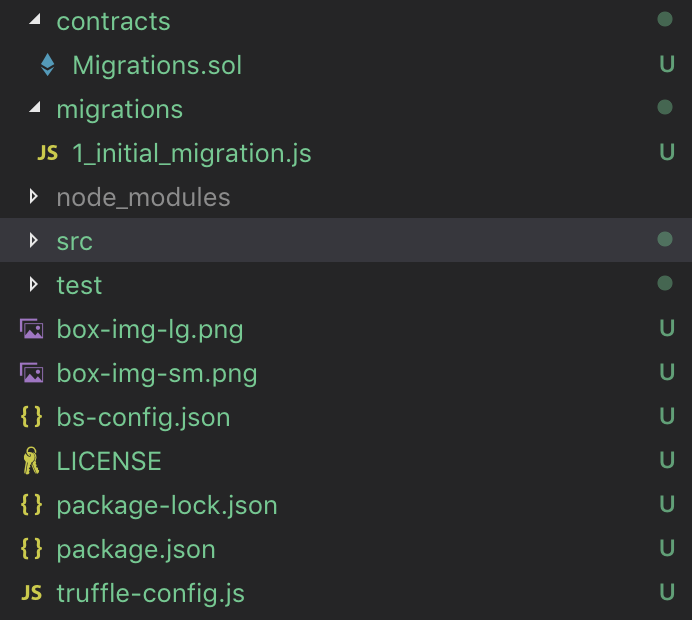
\includegraphics[width=\linewidth/2]{img/truffle-template.png}
		\caption{De structuur van een Ethereum Truffle project}
		\label{fig:truffle-template}
	\end{figure}
	
	\subsection{Basis implementatie}
	We beginnen met het aanmaken van een nieuw smart-contract bestand binnen het template-project. Dit doen we op de locatie \textit{contracts\slash Election.sol}. We overwegen de vereisten voor onze implementatie. Om een simpel stemsysteem te implementeren in een smart-contract hebben we nodig:
	\begin{itemize}
		\item een lijst van de `opties' waarop gestemd kan worden
		\item een lijst van de accounts die gestemd hebben
		\item per optie het aantal stemmen
	\end{itemize}
	Uiteraard zijn er verschillende manieren waarop we dit kunnen aanpakken. In de context van smart-contracts is het echter cruciaal dat we zo weinig mogelijk code schrijven. We baseren ons daarom op de implementatie die wordt gegeven door \textcite{McCubin2019}.\footnote{Zie ook https://github.com/dappuniversity/election}
	
	We beginnen met het declareren van de Solidity versie:

	\lstset{language=JavaScriptSolidity} 
	\begin{lstlisting}[numbers=none]
	pragma solidity ^0.5.8;
	\end{lstlisting}
	\lstset{language=JavaScriptSolidity} 

	Vervolgens starten we met het definiëren we van ons smart-contract \textit{Election} :
	\begin{lstlisting}[numbers=none]	
	contract Election {
		constructor () public {
		}
	}
	\end{lstlisting}
	
	Omdat we een lijst van de `opties' willen hebben en ook per optie willen bijhouden hoeveel stemmen er voor zijn, maken we gebruik van een custom type dat we \textit{Candidate} noemen. 

	Onze verkiezing hoeft niet per se om het verkiezen van een persoon te gaan, het is echter wel handig om over de opties te denken in termen van`kandidaten'. 
	Iedere optie is een kandidaat die een id, een `naam' (de optie tekst) en een aantal voorkeursstemmen heeft. 
	
	In Solidity definiëren we zo'n custom type in de vorm van een \textit{struct}:
	
	\begin{lstlisting}[numbers=none]	
	struct Candidate {
		uint id;
		string name;
		uint votes;
	}
	\end{lstlisting}
	
	We breiden \textit{Election} nu ook uit met de volgende attributen:
	
	\begin{lstlisting}[numbers=none]
	//Fetch the candidates	
	mapping(uint => Candidate) public candidates;
	// Store accounts that have voted
	mapping(address => bool) private voters;
	// Read candidate
	uint public candidatesCounter;
	\end{lstlisting}
	
	Het \textit{mapping} keyword in Solidity duidt een hashTable aan, in Solidity is dit de aangeraden verzameling-structuur\footnote{Zie https://ethereum.stackexchange.com/questions/2592/store-data-in-mapping-vs-array\#answer-2597}.  Mappings laten ons toe om key-value searching te doen. In het geval van  \textit{candiates} mappen we de `kandidaten' op basis van hun id's, die zijn numeriek en incrementeel. We houden het aantal kandidaten bij in \textit{candidatesCounter} zodat we niet onnodig in de mapping moeten zoeken, maar exact weten wat de range van id's is.
	
	Bij het attribuut \textit{voters} mappen we de adressen van alle kiezers op een booleaanse-waarde. Wensen we te weten of een kiezer reeds een stem uitgebracht, dan kunnen we dit via het \textit{voters} attribuut eenvoudig verifiëren. 
	
	We voegen een methode toe aan \textit{Election} die ons instaat stelt om  \textit{candiates} toe initialiseren:
	
	\begin{lstlisting}[numbers=none]
	function addCadidate(string memory _name) private {
		candidatesCounter++;
		candidates[candidatesCounter] = Candidate(candidatesCounter,_name,0);
	}
	\end{lstlisting}
	Merk op dat parameter in de bovenstaande functie gemarkeerd is met het Solidity \textit{memory} keyword. Dit duidt aan dat deze parameter niet in de blockchain dient opgeslagen te worden, de tegenhanger van dit keyword is \textit{storage}.
	
	Voorlopig zullen we onze opties `hardcoden' in de constructor functie, we kiezen voor een implementatie met simpele binaire ja/nee vragen:
	
	\begin{lstlisting}[numbers=none]
	constructor () public {
		addCadidate("Yes");
		addCadidate("No");
	}
	\end{lstlisting}
	
	Nu we opties hebben toegevoegd waarop gestemd kan worden rest ons enkel nog het implementeren van een stem functie. 
	
	Gebruikers mogen niet meermaals een stem uitbrengen, daarom controleren we iedere gebruiker die probeert te stemmen. 
	
	\begin{lstlisting}[numbers=none]
	function hasVoted() public view returns (bool ok) {
		return voters[msg.sender];
	}
	\end{lstlisting}
	
	Merk ook op dat hier wordt gebruik gemaakt van het Solidity \textit{view} keyword, dit duidt aan dat de betreffende functie geen aanpassingen zal maken aan het contract. 
	
	\begin{lstlisting}[numbers=none]
	function vote(uint _candidateId) public {
		if(!hasVoted()) {
			// Record voter has voted
			voters[msg.sender] = true;
			// Update candidate vote count
			candidates[_candidateId].votes++;
		}
	}
	\end{lstlisting}
	
	We vinden de kandidaat waarvoor de gebruiker stemde op basis van de parameter\textit{\_candidateId}. Door deze waarde in te vullen in de mapping \textit{candidates} krijgen we toegang tot de correcte Candidate struct. We verhogen het \textit{votes} attribuut van deze struct met 1. Op dit punt is de stem uitgebracht, we hebben nu een eenvoudig stemsysteem bekomen!
	
	De volledige code voor het smart contract is momenteel:
	
	\lstset{language=JavaScriptSolidity} 
	\begin{lstlisting}[frame=single,  label={lst:election}] 
	pragma solidity ^0.5.8;
	
	contract Election {
		// Store candidate
		struct Candidate {
			uint id;
			string name;
			uint votes;
		}
		
		//Fetch the candidates
		mapping(uint => Candidate) public candidates;
		
		// Store accounts that have voted
		mapping(address => bool) private voters;
		
		// Read candidate
		uint public candidatesCounter;
		
		// Constructor
		constructor () public {
			addCadidate("Yes");
			addCadidate("No");
		}
	
		function addCadidate(string memory _name) private {
			candidatesCounter++;
			candidates[candidatesCounter] = 
			Candidate(candidatesCounter,_name,0);
		}
		
		function hasVoted() public view returns (bool ok) {
			return voters[msg.sender];
		}
		
		function vote(uint _candidateId) public {
			if(!hasVoted()) {
				// Record voter has voted
				voters[msg.sender] = true;
				// Update candidate vote count
				candidates[_candidateId].votes++;
			}
		}
	}

	\end{lstlisting}
	
	
	\subsection{Migration toevoegen}
	Nu we een functioneel smartcontract hebben wensen we dit op onze lokale blockchain te deployen. Hiertoe dienen we  eerst een nieuw migration bestand aan het project toe te voegen op de locatie \textit{migrations\slash 2\_deploy\_contracts.js}.  
	
	Het een nieuwe bestand krijgt de volgende inhoud:
	
	\begin{lstlisting}[frame=single]
	// Find smart contract
	var Election = artifacts.require("./Election.sol");
	
	module.exports = function(deployer) {
	// List all the smart contracts to be deployed
		deployer.deploy(Election);
	};
	\end{lstlisting}
	
	De bovenstaande code zal ervoor zorgen dat Truffle  het `Election' smart contract op de blockchain kan plaatsen wanneer we het project deployen.
	
	\subsection{Truffle project linken aan Ganache}
	
	Om een beter overzicht te krijgen van de `state' van de lokale blockchain kunnen we ons Truffle project in Ganache toevoegen. Dit doen we door binnen Ganche naar de menu-optie `Contracts' te navigeren, vervolgens voor de optie `link truffle  projects'  te kiezen, naar het project te navigeren en daar het bestand \textit{truffle.js} aan te duiden. Tenslotte  kiezen we voor `save and restart'. Als we nu naar de menu-optie `Contracts' gaan krijgen we een overzicht van de contracten en hun status (\ref{fig:contracts-ganache1}).
	
	\begin{figure}
		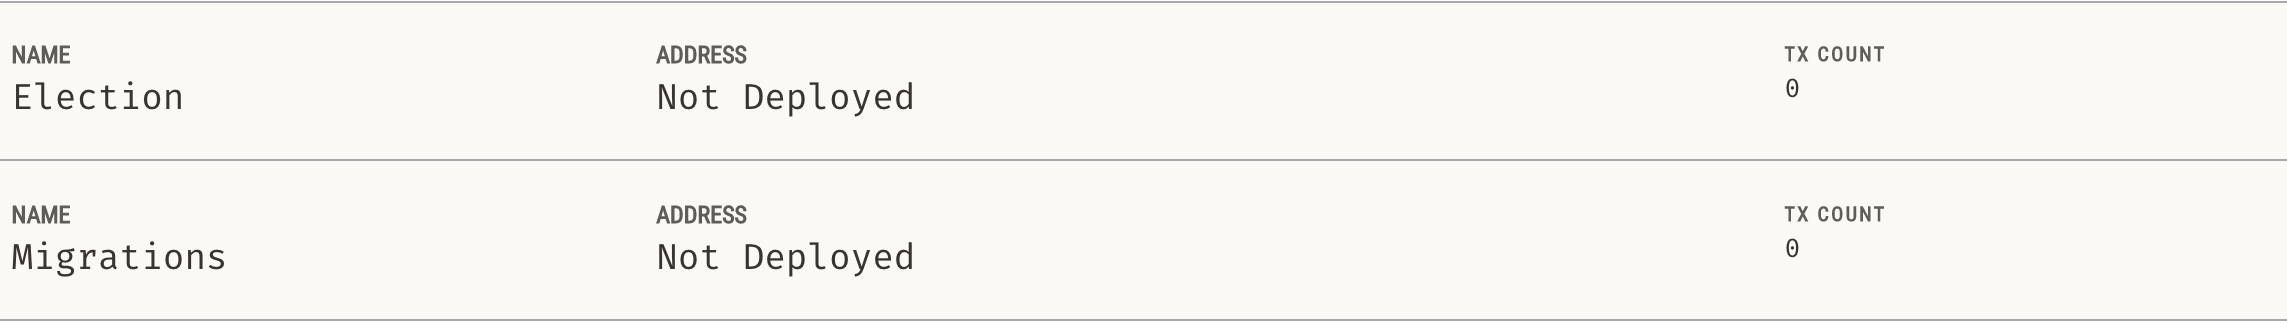
\includegraphics[width=\linewidth]{img/contracts-ganache1.png}
		\caption{De status van smart contracts weergegeven in Ganache}
		\label{fig:contracts-ganache1}
	\end{figure}
	
	
	\subsection{Deployen van smart contracts}
	
	Eenmaal we een migration file hebben voor onze smart-contracts, kunnen we deze deployen. Als de Ganache blockchain opgestart is en het truffle project eraan gelinkt, navigeren we naar het project in de console om vervolgens het volgende console commando te gebruiken:
	
	\begin{lstlisting}[numbers=none]
	> truffle migrate
	\end{lstlisting}
	
	Merk op dat indien we nu opnieuw wensen te deployen (in dit geval niet erg omdat we op een lokale blockchain werken) we het volgende commando dienen te gebruiken:
	
	\begin{lstlisting}[numbers=none]
	> truffle migrate --reset
	\end{lstlisting}
	
	Wanner er geen compilatie fouten aanwezig zijn in de code van de smart contracts kan er met succes deployed worden. In dat geval krijgt men voor ieder van de smart contracts een \textit{transaction receipt}:
	\lstset{language=bash}
	\begin{lstlisting}[numbers=none]
	 Deploying `Election'
	--------------------
	> transaction hash:    0xaf22d8d9c9c9a1230e1764d7a3bd9249a3...eb8fa
	> Blocks: 0            Seconds: 0
	> contract address:    0xBF1917F9c9cFee73A4E653de5ad62a6515b78Ed4
	> block number:        3
	> block timestamp:     1560958652
	> account:             0xE03c3692FED9D4f2cBc7c5a30b05Ae9ce7b3b839
	> balance:             99.98553468
	> gas used:            419914
	> gas price:           20 gwei
	> value sent:          0 ETH
	> total cost:          0.00839828 ETH
	
	
	> Saving migration to chain.
	> Saving artifacts
	-------------------------------------
	> Total cost:          0.00839828 ETH
	\end{lstlisting}
	
	Als we de contracts nu in Ganache bekijken zien we dat de status ook daar veranderd is naar deployed. (Zie Figuur \ref{fig:contracts-ganache2})
	
	\begin{figure}
		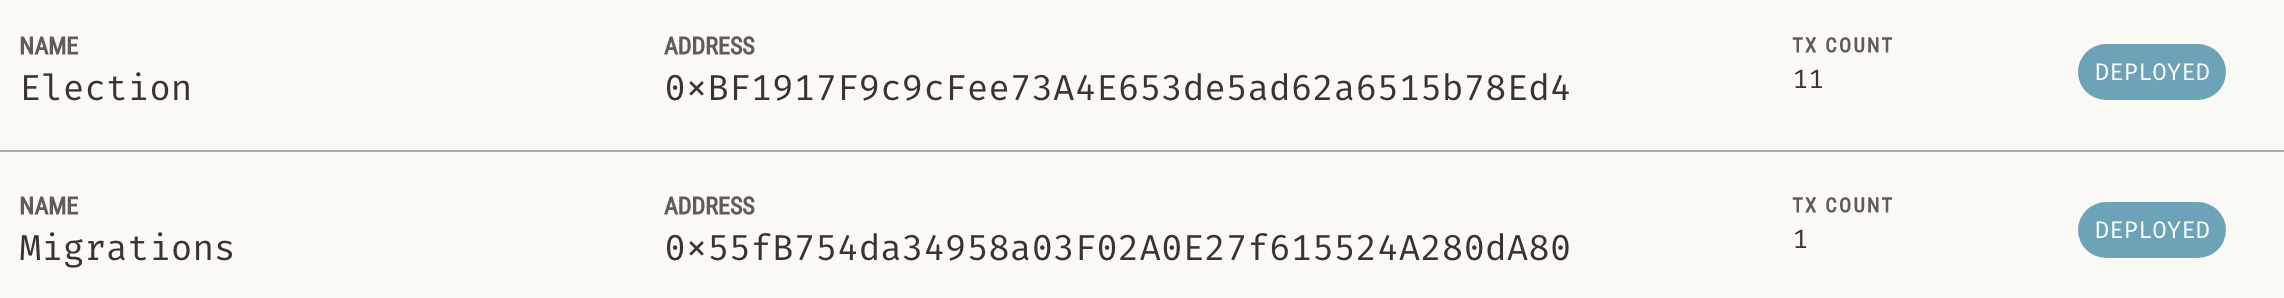
\includegraphics[width=\linewidth]{img/contracts-ganache2.png}
		\caption{Smart contracts deployed weergegeven in Ganache}
		\label{fig:contracts-ganache2}
	\end{figure}
	
	\subsection{Belang van testen}
	Bij het ontwikkelen van dApps speelt testen een cruciale rol. Eenmaal deployed naar een officieel netwerk kunnen functies die bugs bevatten en onverwacht gedrag vertonen erg kostelijk zijn voor gebruikers. Het is daarom best practice om enkel smart contracts te deployen die functioneel-volledig en getest zijn.  Doordat alles wat in de blockchain wordt bewaard immutable is, betekent het herdeployen van een smart-contract eigenlijk dat het huidige contract wordt vervangen door een nieuwe kopie. Zowel de state als het adres van het oude contract gaan verloren. Dit is brekend voor iedere front-end applicatie die aan de dApp verbonden is. 
	
	Door smart-contracts grondig te testen kunnen we dergelijke situaties vermijden.
	
	Er zijn verschillende methoden die men kan toepassen om een smart-contract te testen, standaard is om ze te schrijven in Solidity. Voor dit voorbeeld zullen we echter gebruik maken van Javascript. Via Truffle kunnen we met behulp van Javascript de  interacties van gebruikers met onze smart-contracts gemakkelijk simuleren. Truffle bevat immers standaard Mocha\footnote{Apart verkrijgbaar via https://mochajs.org} (testframework) en Chai Assertion Library\footnote{Apart verkrijgbaar via https://www.chaijs.com}. Deze twee tools stellen ons instaat om onze smartcontracts te importeren binnenin Javascript-testen. 
	
	
	\subsection{Smoke  test}
	We voegen een nieuw bestand toe op de locatie \textit{test\slash election.js}. We schrijven een smoke test, een test die nagaat of het smart-contract op correcte wijze geïnitialiseerd wordt.

	 \lstset{language=JavaScriptSolidity} 
	 \begin{lstlisting}
	 var Election = artifacts.require("./Election.sol");
	 	
	 contract("Election", function(accounts){
		var electionInstance;
		 
		it("Initializes two candidates", function() {
		 	return Election.deployed().then(function(instance){
		 		return instance.candidatesCounter();
		 	}).then(function(count){
		 		assert.equal(count,2);
		 	});
	 	});
	 	
		it("Initializes yes and no", function() {
	 		return Election.deployed().then(function(instance){
	 			electionInstance = instance;
	 			return electionInstance.candidates(1);
	 		}).then(function(candidate){
				assert.equal(
			 	candidate[0],1,"has the correct id: 1"
			 	);
				assert.equal(
				 	candidate[1],"Yes","has the correct value: `Yes'"
				);
				assert.equal(
				 	candidate[2],0,"has the correct amount of votes: 0"
				);
				return electionInstance.candidates(2);
	 		}).then(function(candidate){
				assert.equal(
					candidate[0],2,"has the correct id: 2"
				);
				assert.equal(
					candidate[1],"No","has the correct value: `No'"
				);
				assert.equal(
					candidate[2],0,"has the correct amount of votes: 0"
				);				
	 		}); // End function
	 	}); // End it()
	}); // End contract
	\end{lstlisting}
	
	Concreet testen we hier dat na instantiatie:
	\begin{itemize}
		\item Het attribuut \textit{canidatesCounter} = 2 is.
		\item Het attribuut \textit{candiates[0]} een `kandidaat' is met id = 1, naam = ``Yes'' en aantal stemmen = 0.
		\item Het attribuut \textit{candiates[1]}  een `kandidaat' is met id = 2, naam = ``No'' en aantal stemmen = 0.
	\end{itemize}
	\subsection{Testen uitvoeren}
	Om geschreven testen uit te voeren navigeren we naar de project-directory en gebruiken we het console commando:
	
	\begin{lstlisting}[numbers=none]
	> truffle test
	\end{lstlisting}
	
	Truffle voert hierop de al de testen binnen de directory \textit{test\slash} uit:
	
	\begin{lstlisting}[numbers=none]
	> Artifacts written to /var/folders/xq/mnnky8qn6c58pt33xhpz2bhw0000gn/T/test-119519-4744-y0zb1c.1il0l
	> Compiled successfully using:
	- solc: 0.5.8+commit.23d335f2.Emscripten.clang
	
	
	
	Contract: Election
	v Initializes two candidates
	v Initializes yes and no (93ms)
	
	
	2 passing (173ms)
	\end{lstlisting}
	
	De smoke test slaagt.
	
	\subsection{Testen in de Truffle console}
	Uiteraard dienen we  ook testen te schrijven voor de stem-functionaliteit. Gezien dit onderdeel van de code echter nog aan veranderingen onderworpen zal worden is het misschien voordeliger om de huidige werking op een andere manier te verifiëren. In plaats van een test te schrijven, kunnen we via de \textit{Truffle console} de toestand van de lokale blockchain bekijken.
	
	In de console navigeren we naar het project, vervolgens gebruiken we het console commando:
	
	\begin{lstlisting}[numbers=none]
	> truffle console
	\end{lstlisting}
	
	Dit opent de Truffle console. 
	Hier geven we het volgende commando in:

	\begin{lstlisting}[numbers=none]
	truffle(development)> Election.deployed()
		.then(function(i){app = i})
	\end{lstlisting}
	
	Indien het Election contract deployed is, wordt er een asynchrone callback-functie uitgevoerd.  De functie in kwestie krijgt  een instantie van Election (i) mee als parameter en maakt deze toegankelijk door ze in hem variabele op te slaan.
	Eenmaal de asynchrone code uitgevoerd is, hebben we via \textit{app} toegang tot de attributen en functies van het smart contract Election.
	
	Gezien we de stemfunctionaliteit willen testen, zullen we de stemfunctie \textit{vote()} oproepen.
	
	Hiervoor hebben we echter het publieke adres van één van de Ganache accounts nodig. Deze adressen kan men vinden in Ganache zelf, of bekomen via het Truffle console commando:
	\begin{lstlisting}[numbers=none,language=bash]
	truffle(development)>web3.eth.getAccounts()
	[ `0xE03c3692FED9D4f2cBc7c5a30b05Ae9ce7b3b839',
	`0xe60c19f8a1baC541483e303Dc3d9B4e28d580980',
	`0x47B7B70802E9eC6a5Df8570962574894f0Ac4c15',
	`0xE4978a5B03C37245356c1dFdBBc536093aA4887d',
	`0xeA48794bF89B626392FF85ec9786671286B4a0c4',
	`0x4C57CA30fa4Ba94066bb65F180B87438566400b7',
	`0xb6997ce4fdE3C0D3002C6A6208AB60cd0CF2c1aA',
	`0xa9a71102f482960839b85d389C553fDa69e603F4',
	`0xd99Fe17d5Dc01aDfd691DA97E056979C8ADBefa7',
	`0xa12D538888E90A2DA7763Bd8F64595e568c3dFE0' ]
	\end{lstlisting}
	
	We kopiëren een adres naar keuze en vullen dit in als \textit{from} property van de 2e parameter. Op deze manier versturen we een transactie vanuit de console, in naam van het geselecteerde adres. De 1e parameter is het id van de `kandidaat' waarvoor we stemmen.
	\begin{lstlisting}[numbers=none,language=bash]
	truffle(development)> app.vote(1,
		{ from: `0xE03c3692FED9D4f2cBc7c5a30b05Ae9ce7b3b839'}
	)
	\end{lstlisting}
	
	Ook hier krijgen we een \textit{transaction receipt.} Ook in Ganache zien we dat er een  nieuwe transactie heeft plaats gevonden (Figuur \ref{fig:contracts-ganache3})
	\begin{figure}
		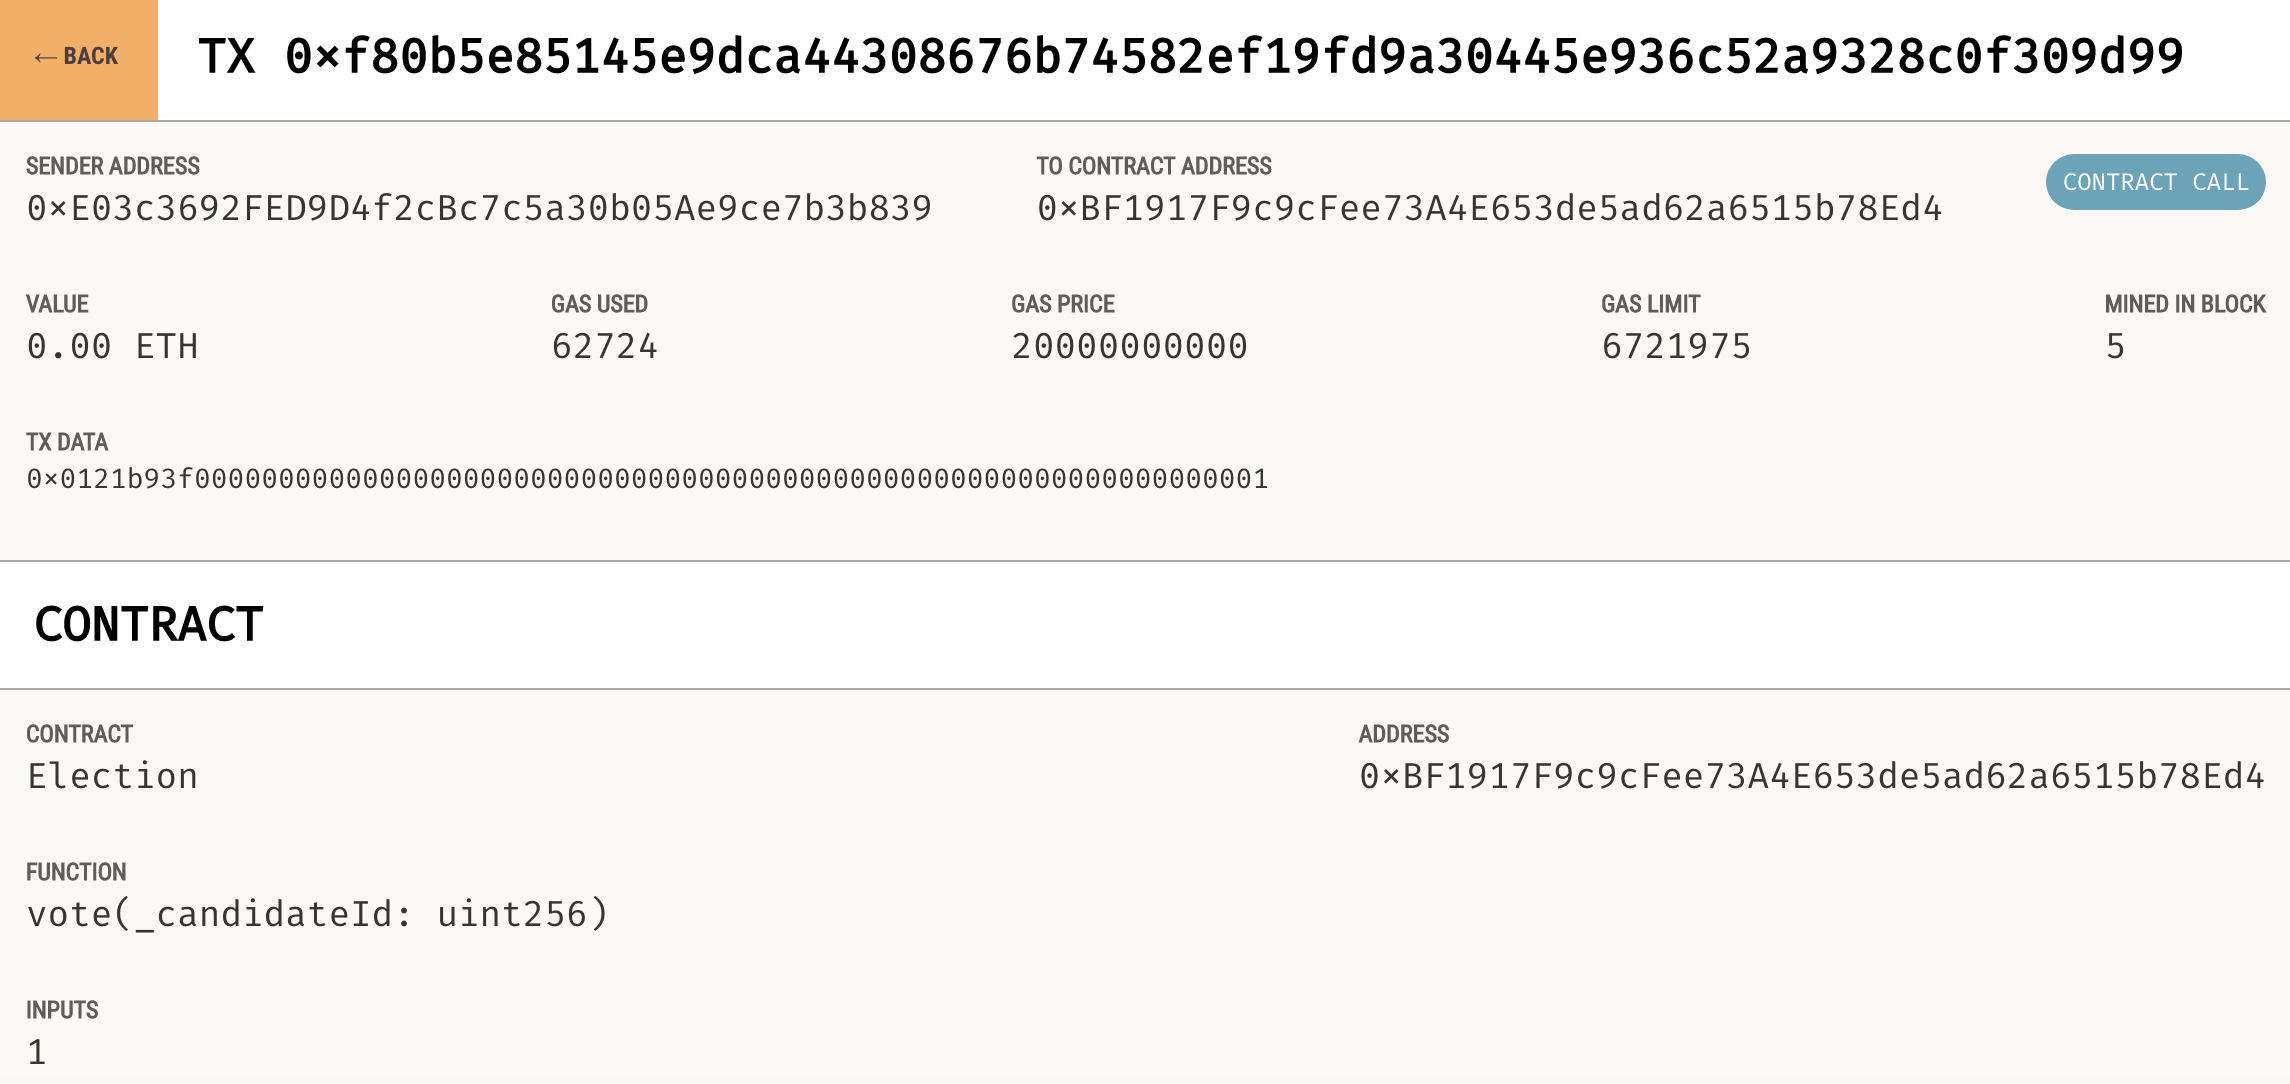
\includegraphics[width=\linewidth]{img/contracts-ganache3.png}
		\caption{Vote functie aangeroepen weergegeven in Ganache}
		\label{fig:contracts-ganache3}
	\end{figure}
	Om te controleren of er een stem is bijgekomen voor de gekozen optie geven we de volgende Truffle console commando's in:
	\begin{lstlisting}[numbers=none]
	truffle(development)> app.candidates(1)
	truffle(development)> app.candidates(2)
	\end{lstlisting}
	
	Dit resulteert in:
	\begin{lstlisting}[numbers=none,language=bash]
	Result {												Result {
	...															...
	id: <BN: 1>,										id: <BN: 2>,
	name: `Yes',									  name: `No',
	votes: <BN: 1> }							  votes: <BN: 0> }
	\end{lstlisting}
	
	Voor de eerste optie (`Yes') zien we dat er onder het attribuut \textit{votes} de waarde <BN: 1> staat. Het aantal stemmen hier is met andere woorden 1.
	Voor de tweede optie (`No') is dat niet het geval, \textit{votes} heeft de  waarde <BN: 0>. Het aantal stemmen hier dus onveranderd, 0.
	
	Dit toont aan dat onze stem-functie wel degelijk werkt!
	
	Merk wel op dat in de huidige implementatie totaal geen garantie biedt op het vlak van anonimiteit. Het enigste wat de anonimiteit van een kiezer enigszins beschermt is de abstracte aard van accounts, de kiezer is alleen bekend via zijn Ethereum adres. 
	
	\subsection{Ethereum en geheimen bewaren}
	Een van de moeilijkheden waarmee men te maken krijgt tijdens ontwikkelen van gedecentraliseerde applicaties binnen Ethereum, is het feit dat het zeer moeilijk is om anonimiteit of privacy voor gebruikers te creëren. De aard zelf van de blockchain-technologie legt immers de nadruk op het publiek beschikbaar maken van alle gegevens. In Ethereum zien we dit zeer sterk, iedere transactie en al de daar bijhorende parameters zijn publiek.  Bovendien gaat het veel verder dan alleen transacties. Eigenlijk is alles publiek binnen de Ethereum-blockchain. Private attributen en methoden mogen dan wel bestaan, de waarden zullen nog steeds publiek zichtbaar zijn. \autocite{Buterin2014}
	
	Voor onze implementatie vormt dit een potentieel probleem, gezien we een stem als parameter wensen door te geven. Op het vlak van stemsystemen is anonimiteit van kiezers  vaak noodzakelijk. Gezien Ethereum geen private transacties ondersteund (sommige blockchains doen dit wel)  moeten we op zoek gaan naar alternatieve methodes. Het lijkt een logische om te kijken of we de stem van de kiezer die we doorgeven als parameter niet kunnen encrypteren. Het probleem is echter dat standaard encryptie en decryptie technieken niet zullen werken op de blockchain. We kunnen immers geen enkel geheim bewaren op de blockchain,  decryptie sleutels zijn dus ook onmogelijk.
	
	Het gevolg is dus dat we geen keuze hebben dan gebruik moeten maken van  geavanceerde cryptografische technieken, willen we ons systeem volledig veilig maken. Een mogelijke cryptografische techniek de we hier zouden kunnen toepassen is die van het OVNP van \textcite{McCorry2017} dat we in het vorige hoofdstuk bespraken. Dit blijkt echter in de praktijk zeer moeilijk te doen. In een volgende sectie zullen we hier verder op ingaan.	
	
	\begin{figure}
		\centering
		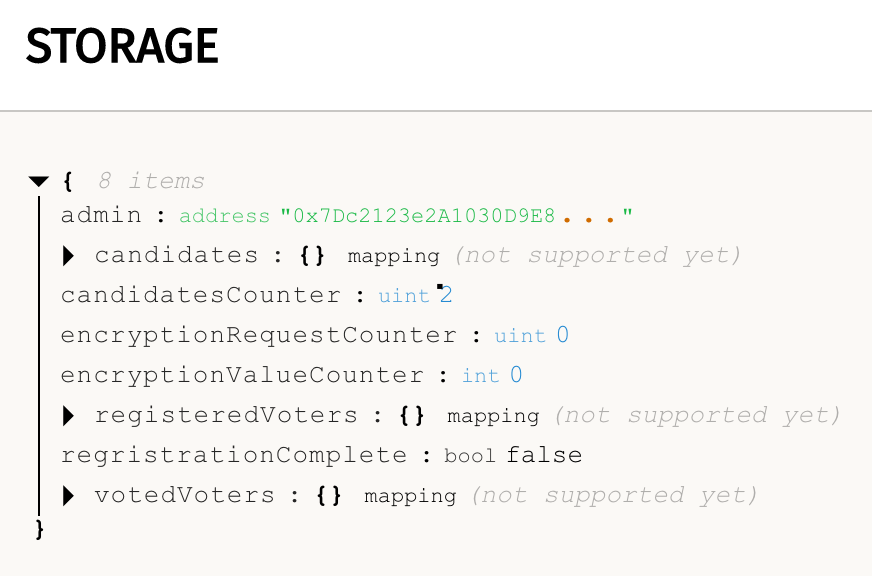
\includegraphics[width=\linewidth/2]{img/contracts-ganache4.png}
		\caption{Alle attributen van een contract zijn publiek zichtbaar}
		\label{fig:contracts-ganache4}
	\end{figure}

	\section{Front-end applicatie}
	Eenmaal we de basis we een werkende basis back-end hebben dienen we er natuurlijk ook nog een front-end applicatie voor te ontwikkelen. In deze handleiding zullen we gebruik maken van een Angular, een open source javascript-framework dat de ontwikkelaars instaat stelt om performante Single Page Applications te schrijven. We maken gebruik van Angular omdat de structurering  van de code bijzonder regide is, waardoor de functionaliteiten mooi opgesplitst zijn en de ontwikkelervaring bijzonder aangenaam.  Het staat de lezer echter vrij om een javascript-framework naar keuze te gebruiken, indien hij of zij dat wenst. Het gaat hier  niet zo zeer om de ontwikkeling van de front-end applicatie als om het maken van de verbinding tussen webapplicatie en Ethereum blockchain zodat we kunnen interageren met ons smart-contract. 
	
	\subsection{Opzet}
	Zoals gezegd zullen we een Angular project opzetten, lezers die gebruik wensen te maken van een ander Javascript-framework kunnen de komende stappen overslaan, zij hoeven enkel de vernoemde \textit{node\_modules } te installeren. 
	
	We beginnen met het installeren van de angular cli, deze zal ons toe laten om een angular project te maken.
	
	maken gebruik van het console commando:
	\begin{lstlisting}[numbers=none,language=bash]
	>npm install -g @angular/cli
	\end{lstlisting}
	Dit installeert de angular cli op een globaal niveau, vanaf nu kunnen we er overal gebruik van maken.
	
	We navigeren naar de directory waar we het front-end project willen aanmaken, vervolgens gebruiken we het console commando:
	\begin{lstlisting}[numbers=none,language=bash]
	>ng new EthereumVote
	\end{lstlisting}
	De angular cli zal nu een nieuw project voor ons creëren in de huidige directory. 
	
	Nu installeren we de nodige node\_packages:
	\begin{itemize}
		\item \textbf{web3.js}: een verzameling javascript libraries  die toelaten om te communiceren met Ethereum-instantie, hetzij via  een HTTP-, WebSocket- of IPC-verbinding.
	\end{itemize}
	
	
	
	
	
	
	Navigeer naar de hoofddirectory van het nieuwe project en maak een nieuwe directory `services':
	\begin{lstlisting}[numbers=none,language=bash]
	>mkdir services
	\end{lstlisting}
	Navigeer vervolgens naar die directory en 
	
	
	
	
	
	
	
	
	
	
	
	
	
	
	
	
	

	








